\documentclass[e2_tp1_main.tex]{subfiles}

\begin{document}

\section{Caracter\'istica de salida}


Se realizaron mediciones de la tensi\'on y la corriente de salida para distintos valores de carga, obteni\'endose as\'i las curvas caracter\'isticas del circuito. Las mismas se realizaron para tres tensiones de regulaci\'on distintas: 9V (figura \ref{fig:cs9}), 12V (figura \ref{fig:cs12}) y 15V (figura \ref{fig:cs15}).

\begin{figure}[!htb]
	\centering
	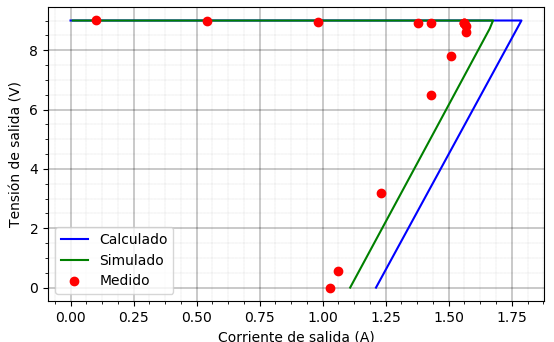
\includegraphics[width=0.8\textwidth]
	{curvas_salida/e2_tp1_carac_salida_9V.png}
	\caption{Curva de salida calculada, simulada y medida, con $V_O|_{REG}=9$V}
	\label{fig:cs9}
\end{figure}



En las mediciones, se observa que la tensi\'on de corto circuito real fue menor a la simulada, que a su vez fue menor a la calculada. Recordando la expresi\'on de esta corriente:
\[ I_{O\, CC} = 	\left( \frac{V_{BE\, 4}}{R_4} \right) \cdot
				\left( 1 + \frac{R_2}{R_3} \right)\]

De aqu\'i resulta evidente que esta corriente depende considerablemente de la polarizaci\'on de $T_4$. Si bien en los c\'alculos se consider\'o $V_{BE}=0.7$V, en la simulaci\'on se observa que esta tensi\'on es de 0.65V, lo cual reduce el valor de $I_{O\,CC}$ un 7.14\%: de 1.2A a 1.11A, lo cual explica la diferencia entre el c\'alculo y la simulaci\'on. En cuanto a la diferencia entre la simulaci\'on y la medici\'on, puede atribuirse el error obtenido a la tolerancia de los componentes (sobre todo de $R_2$, cuya sensibilidad es particularmente alta, dado que $R_2$ es considerablemente menor a $R_3$).

Otra diferencia notable entre la curva calculada y las demas est\'a en la ca\'ida de tensi\'on que se observa en la salida incluso antes de entrar en foldback. Los cambios peque\~nos que se observan para corrientes menores a 1.5A se pueden atribuir a que la impedancia de salida no es exactamente 0, y por lo tanto la regulaci\'on de l\'inea no es del todo perfecta.  Pero para corrientes superiores, se comienza a observar un descenso mayor en la tensi\'on. Esto se debe a que la protecci\'on no se activa para un valor concreto de corriente, como se modeliza, si no que $T_4$ pasa gradualmente de corte a modo activo.

\begin{figure}[!htb]
	\centering
	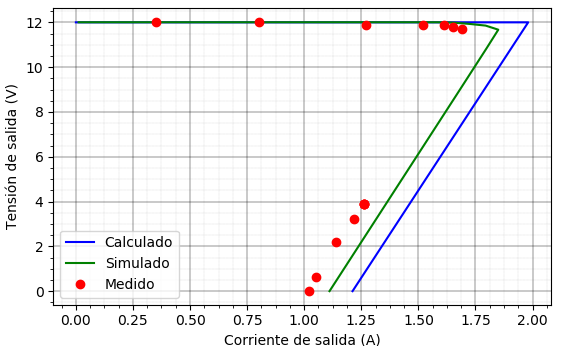
\includegraphics[width=0.8\textwidth]
	{curvas_salida/e2_tp1_carac_salida_12V.png}
	\caption{Curva de salida calculada, simulada y medida, con $V_O|_{REG}=12$V}
	\label{fig:cs12}
\end{figure}


\begin{figure}[!htb]
	\centering
	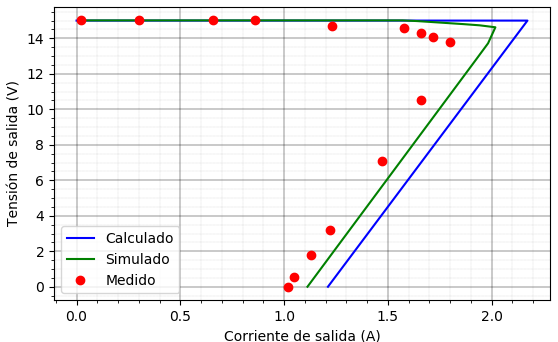
\includegraphics[width=0.8\textwidth]
	{curvas_salida/e2_tp1_carac_salida_15V.png}
	\caption{Curva de salida calculada, simulada y medida, con $V_O|_{REG}=15$V}
	\label{fig:cs15}
\end{figure}


\end{document}